\section{The Unicycle Model}
The unicycle model is a planar model of a robot having two wheels placed at a distance $d \in \mathbb{R}$ with a coinciding rotation axis (Figure~\ref{fig:notation}).  As a consequence, this mobile robot cannot move sideways, along the wheel axis, but it can turn by moving the wheel at different velocity. 

In this section we are going to use the following notation:
\begin{itemize}
	\item The $i_{th}$ component of a vector $x$ is denoted as $x_i$~and, for the sake of brevity, 
	$x_1 \vec{u} {+} x_2 \vec{w}$ is written as $(\vec{u},\vec{w})x$.
	
	\item $\mathcal{I} = \{O;\vec{\imath}_0,\vec{\jmath}_0\}$ is a fixed inertial frame with respect to (w.r.t.) 
	which the robot's absolute pose is measured.
	\item The point $M$ is the middle point of the wheel's axis, and $\mathcal{B} = \{M; \vec{\imath}, \vec{\jmath}\}$ is a frame attached to the robot.
	The vector $\vec{\imath}$ is perpendicular to the  wheel's axis.  
	% This leaves two possible (and opposite) directions for this vector.
	% The direction chosen here is consistent with a \emph{forward} direction associated with the robot.
	%\item The position of the robot is given by the geometric vector $\vec{OM}$ whose coordinates w.r.t. the inertial frame are 
	%defined by $\vec{OM} = (\vec{\imath}_0,\vec{\jmath}_0) x $. 
	\item $F$ denotes a point attached to the robot. Then, $\vec{OF} = (\vec{\imath}_0,\vec{\jmath}_0) x_f $ and 
	$\vec{MF} =  (\vec{\imath},\vec{\jmath}) d$, with $d$ a constant vector.
	%\item The point $P$ represents the position of a person. 
	%Then, $\vec{OP} = (\vec{\imath}_0,\vec{\jmath}_0) x_{p}$ and the velocity of the person is defined by $\vec{v}_p := \tfrac{d}{dt}\vec{OP} = (\vec{\imath}_0,\vec{\jmath}_0) \dot{x}_p$.
	\item $e_1 := (1,0)^T$ and $e_2 :=(0,1)^T$ denote the canonical basis vectors of $\mathbb{R}^2$.
	\item The rotation matrix of an angle $\theta$ is denoted as $R(\theta)$; $S=R(\pi/2)$ is the unitary skew-symmetric matrix, i.e.
	\[
	R(\theta)= \begin{pmatrix}
	\cos \theta & - \sin \theta \\
	\sin \theta & \cos \theta
	\end{pmatrix} \, , \quad 
	S =  \begin{pmatrix}
	0 & -1 \\
	1 & 0
	\end{pmatrix}.
	\]
\end{itemize}

\begin{figure}[tpb]
	\centering
	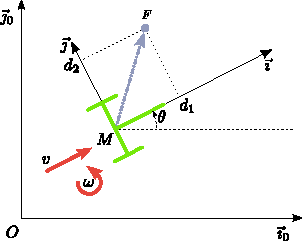
\includegraphics[width=.5\textwidth]{figures/notation_simple.pdf}
	\caption{Notation.}
	\label{fig:notation}
\end{figure}

The model equations are the following \cite{pucci2013nonlinear}:
\begin{IEEEeqnarray}{RCL}
	\IEEEyesnumber
	\dot x & = & v R(\theta) e_1, \IEEEyessubnumber \label{honolonimicCon} \\
	\dot \theta & = & \omega,       \IEEEyessubnumber
\end{IEEEeqnarray}
with $v$ and $\omega$ the robot's rolling and rotational velocity, respectively. 
The variables $v$ and $\omega$ are considered 
as kinematic control inputs.

\subsection{Unicycle Controller}
The control objective is to asymptotically stabilize the point $F$ about a desired point $F^*$. For this purpose, 
define the coordinates of the geometric position error $\vec{FF^*}$ as follows 
\begin{eqnarray}
\vec{FF^*} = (\vec{\imath}_0,\vec{\jmath}_0)\tilde{x},  \nonumber
\end{eqnarray}
so that
\begin{equation}
\tilde{x}  := x_f - x_f^*. \label{eq:xtilde}
\end{equation}
Then, the control objective is equivalent to the asymptotic stabilization of $\tilde{x}$ to zero.
Since
\[ x_f = x + R(\theta)d,\]
then differentiating Eq. \eqref{eq:xtilde} yields 
\begin{IEEEeqnarray}{RCL}
	\IEEEyesnumber
\dot{\tilde{x}} &=& \dot{x} + \dot{R}(\theta)d \IEEEyessubnumber \\
&=& \dot{x} + \omega R(\theta) S d. \IEEEyessubnumber
\end{IEEEeqnarray}
Notice that 
\begin{IEEEeqnarray}{RCL}
	R(\theta) &=& \begin{pmatrix}
		\cos \theta & - \sin \theta \\
		\sin \theta & \cos \theta 
	\end{pmatrix} \nonumber \\
	\dot{R}(\theta) &=& \begin{pmatrix}
		\sin \theta & - \cos \theta \\
		\cos \theta & - \sin \theta 
	\end{pmatrix}\omega \nonumber \\
	&=& \begin{pmatrix}
		\cos \theta & - \sin \theta \\
		\sin \theta & \cos \theta 
	\end{pmatrix} 
	\begin{pmatrix}
		0 & - 1 \\
		1 & 0
	\end{pmatrix}\omega \nonumber\\ 
	 &=& R(\theta)S = SR(\theta). \nonumber
\end{IEEEeqnarray}



with 
\[ M :=  \left[ \begin{array}{cc} 1 & -d_2 \\ 0 & d_1 \end{array} \right], \quad u := \left[ \begin{array}{c} v 
\\ \omega \end{array} \right], \quad \vr := \rtm^T \xrd. \]

Classical control laws that asymptotically stabilize $\tilde{p} = 0$ when the point $F$ is not along the wheels' axis, i.e. $d_1\ne 0$.
\begin{lemma}
	\label{lem:pfmneq0}
	Assume that $d_1 \neq 0$ so that $\text{det}(M) \neq 0$. Apply the control
	input
	\begin{eqnarray}
	u & = &  M^{-1} \left[\vr - K \tilde{p} \right],
	\label{eq:posparamctrl}
	\end{eqnarray}
	to System \eqref{eq:ptd} with \[K= \left[ \begin{array}{cc} k_1 & 0 \\ 0 & k_2 \end{array} \right], \quad K > 0.\]
	Then,
	\begin{eqnarray}
	\dot{\tilde{p}} = - \omega S \tilde{p} - K \tilde{p},
	\end{eqnarray}
	and $\tilde p=0$ is a globally asymptotically stable equilibrium point for the closed-loop system.
\end{lemma}

$\\$
This result ensures that when the control point $F$ is not located on the wheels' axle, its stabilization to an arbitrary 
reference position $P$ can be achieved by the use of simple feedback laws. This control strategy works very well when~$F$ 
is located ahead of the  wheels' axle, 
% i.e. $|d_1/d_2| \gg 1$, 
which 
corresponds to the situation where the robot follows the user. Several limitations of
this approach, however, must be mentioned. For instance, the control law is not defined when~$F$ is located on the wheel's axle
and this gives rise to ill-conditioning problems when $F$ is close to this axle (the matrix $M$ is close to singular). 
Still, this situation is of practical interest for many applications where the user wants to remain close to the platform and keep it in his/her 
field of view. Another drawback of the control \eqref{eq:posparamctrl} is that when the 
robot is located behind the user, it tends to turn back if the user starts moving backward  
--~this is the so-called  \emph{jack-knife effect}. We present below a new feedback control law to address these 
problems when $F$ is located on the wheels' axle.
